\section{Performantie}
\label{sec:evaluatie-performantie}

Eerst zal de totale performantie worden besproken van de vier raamwerken.
Daarna zal in sectie~\ref{sec:evaluatie-downloadtijd} de gemiddelde downloadtijd gedetailleerd worden besproken.
Hieropvolgend zal in sectie~\ref{sec:evaluatie-gebruikerservaring} de gebruikerservaring worden besproken.
Als laatste wordt de performantie getoetst aan andere metrieken in sectie~\ref{sec:evaluatie-performantie-xxx}.

Vooral de totale performantie kan besproken, zal de formule om de totale performantie te berekenen~(zie \ref{eq:performantie}), moeten worden herschreven.
Dit komt doordat in de gebruikerservaring zal worden vervangen door een subjectieve lijsttest (zie \ref{sec:evaluatie-gebruikerservaring}). 
De opzet van de nieuwe formule is om een raamwerk dat slecht scoort op gemiddelde downloadtijd, maar sterk scoort op de subjectieve lijsttest, een middelmatige score te geven.
Aangezien deze laatste geen eenheid heeft en de eerstgenoemde uitgedrukt wordt in seconden, wordt de downloadtijd gedeeld door de gebruikerservaring. De score voor de performantie van een raamwerk $r$ wordt:
\begin{equation}
  \text{Performantie}'_r = \frac{\text{Totale downloadtijd}_r}{\text{Totale gebruikerservaring}'_r}
  \label{eq:performantie-enhanced}
\end{equation}

De bekomen data voor de vier raamwerken aan de hand van deze nieuwe formule wordt weergegeven in tabel \ref{tabel:evaluatie-performantie}.

\begin{table}[H]
\centering
\pgfplotstabletypeset[
  begin table=\begin{tabular}{p{8cm} p{0.8cm} p{0.8cm} p{0.8cm} p{0.8cm} p{0.3cm}},
  end table=\end{tabular},
  skip coltypes=true,
  col sep=comma,
  string type,
  header=true,
  columns={Performantie,ST,Kendo,jQM,Lungo},
  columns/Performantie/.style={column name=\textbf{Performantie}, column type={l}},
  columns/ST/.style={column name=\textbf{\sta}, column type={l}},  
  columns/jQM/.style={column name=\textbf{\jqma}, column type={l}},    
  columns/Kendo/.style={column name=\textbf{\kendoa}, column type={l}},   
  columns/Lungo/.style={column name=\textbf{\lungoa}, column type={l}}, 
  every head row/.style={
    before row=\toprule,
    after row=\midrule},
  every last row/.style={
  	before row=\midrule,
    after row=\bottomrule}
]{tabellen/performantie.csv}
\caption{Overzicht van performantie voor \st{}~(\sta), \kendo{}~(\kendoa), \jqm{}~(\jqma) en \lungo{}~(\lungoa). Minder is beter.}
\label{tabel:evaluatie-performantie}
\end{table}

%TODO Tim: ik heb zelf dit besluit getrokken, klopt het? nog opmerkingen?
Het is duidelijk dat op vlak van totale performantie \jqm{} het beste scoort, kort gevolgd door \lungo{}.
Dit wordt verklaard doordat deze raamwerken geen architectuur afdwingen waardoor er ook een kleinere \js{}-code dient te worden gedownload ten opzichte van raamwerken die wel een architectuur afdwingen (zie ook tabel \ref{tabel:raamwerken-tabel}).
\kendo{} en \st{} komen respectievelijk op de voorlaatste en laatste plaats.

%%%%%%%%%%%%%%%%%%

\subsection{Gemiddelde downloadtijd}
\label{sec:evaluatie-downloadtijd}

Op figuur \ref{fig:performantie} wordt de gemiddelde downloadtijd van de POC en login, zowel gewoon als uit cache, voor de vier raamwerken getoond.
Voor de gemiddelde downloadtijd per apparaat per raamwerk wordt verwezen naar appendix \ref{app:performantie}.

\begin{figure}[H]
  \centering
  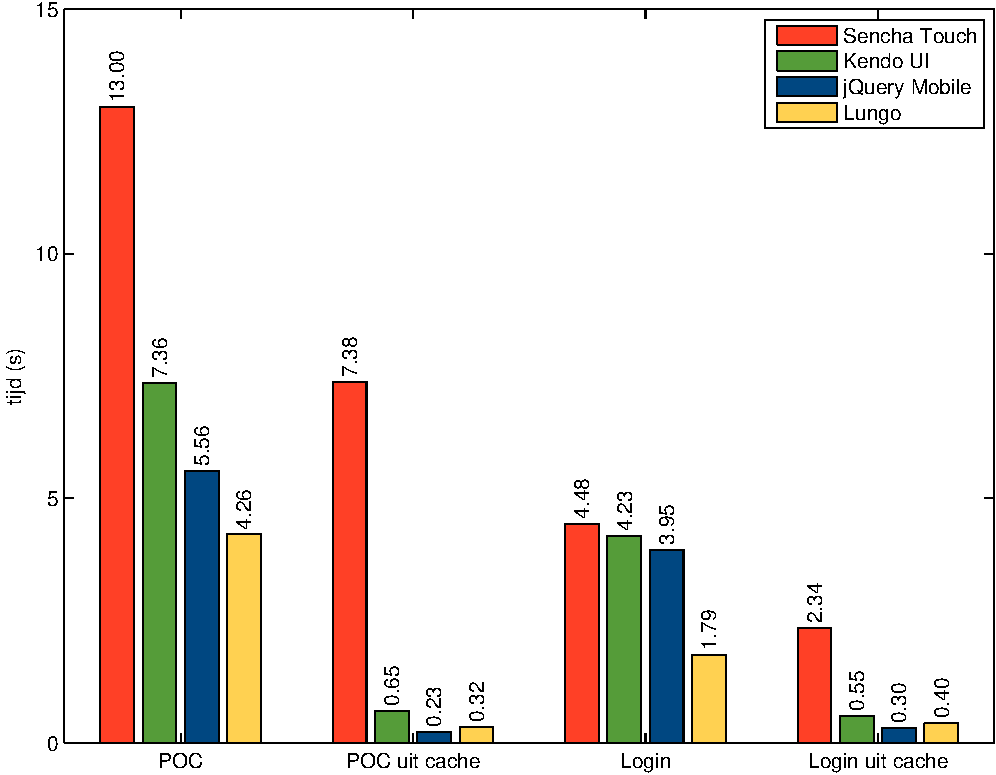
\includegraphics[width=\textwidth]{figuren/performance.pdf}
  \caption{Gemiddelde downloadtijd van POC,  POC uit cache,  login en login uit cache voor elk raamwerk. Minder is beter.}
  \label{fig:performantie}
\end{figure}

\lungo{} behaalt de eerste plaats.
Als er gekeken wordt naar de POC heeft \lungo{} maar een derde van de tijd nodig ten opzichte van het traagste raamwerk, \st.
\jqm{} en \kendo{} behalen respectievelijk een tweede en derde plaats.
Aangezien niet alles werd geïmplementeerd in de POC voor \lungo{}, zou kunnen worden gesteld dat dat de reden is.
Als er echter wordt gekeken naar de loginapplicatie waar alles wel vergelijkbaar is, dan blijft \lungo{} het snelste raamwerk.
Het is zelfs meer dan de helft sneller dan \jqm{}, \kendo{} of \st{}.
Deze drie raamwerken behalen quasi dezelfde opstarttijd.
\kendo{} en \st{} nemen respectievelijk voorlaatste en laatste plaats in.
Dit wordt verklaard door het gebruik van een architectuur waardoor een grotere \js{}-code dient te worden gedownload ten opzichte van raamwerken die geen architectuur afdwingen (zie ook tabel \ref{tabel:raamwerken-tabel}).

Als naar de versie uit cache wordt gekeken voor zowel POC als loginapplicatie, scoren \kendo{}, \jqm{} en \lungo{} hetzelfde.
Daarentegen behaalt \st{} telkens een vele tragere tijd.
Enerzijds komt dit doordat de drie eerstgenoemde raamwerken enkel gebruik maken van HTML5 Application Cache.
\st{} gebruikt daarnaast ook nog een eigen mechanisme waardoor de grotere laadtijd wordt verklaard (zie \ref{app:performantie-st}).
Anderzijds gebruiken de drie eerstgenoemde raamwerken Yeoman om de applicatie te bouwen.
De webapplicaties gemaakt \st{} gebruiken daarentegen Sencha Cmd.

%%%% De cache factor van ST is constant (gemiddeld 1,8)
%%%% De andere raamwerken hebben een beduidend grotere cache factor 

Indien \st{} buiten beschouwen wordt gelaten, duurt het eerste keer laden van de POC gemiddeld 5,73 seconden. 
Het laden van de versie uit cache duurt slechts gemiddeld 400 milliseconden.
De eerste keer laden van de loginapplicatie duurt gemiddeld 3,32 seconden.
Indien deze uit cache komt, duurt dit nog slechts gemiddeld 420 milliseconden.
Dit zijn aanvaardbare tijden volgens Jakob Nielsen~\cite{Nielsen1993} doordat de tijden uit cache onder de seconde blijven.
Volgens Nielsen dient er wel feedback over het laden te worden gegeven aan de gebruiker.
Dit neemt de browser voor zich door bij het laden een laadbalk of spinner te tonen.

%%%%%%%%%%%%%%%%%%

\subsection{Gebruikerservaring}
\label{sec:evaluatie-gebruikerservaring}
De gebruikerservaring via \js{} kon enkel worden opgemeten in \jqm{} en \kendo{}.
Bij de twee andere raamwerken werden de betreffende \term{events} niet gevonden om correct de tijd op te meten.
% TODO: eventueel referenties naar vragen op so
Doordat er maar data voor twee raamwerken voor handen was, werd deze methode vervangen door een subjectieve lijsttest.
Deze bestaat eruit de vlotheid van het scrollen door de lijst van 850 lijstelementen voor de vier raamwerken op de 8 apparaten te vergelijken.
Per apparaat word een score van 1, 2, 3 of 4 uitgedeeld aan de raamwerken.
Hierbij is 4 de beste score wat overeenkomt met het vlotste scrollen door de lijst relatief ten opzichte van de drie andere raamwerken.
Deze test werd uitgevoerd door twee personen.
% TODO: is dat nu goed of slecht als we dat maar met 2 personen hebben gedaan?
%Er dient echter opgemerkt te worden dat het tijdsbudget het niet toeliet om deze test te laten uitvoeren door minstens vijf personen te laten uitvoeren, wat voorgesteld wordt door Nielsen.

Om de totaalscore van een raamwerk te bepalen worden de scores voor dat raamwerk op ieder apparaat opgeteld. De nieuwe formule voor totale gebruikerservaring voor een raamwerk $r$ wordt:
\begin{equation}
  \text{Totale gebruikerservaring}'_r = \sum_{c=1}^{8}{\text{ervaring}_{r,c}}
  \label{eq:performantie-enhanced}
\end{equation}

In het bekomen eindklassement komt de hoogste totaalscore overeen met het raamwerk dat de vlotste scrolervaring aanbiedt. In tabel \ref{tabel:evaluatie-performantie-gebruikerservaring} wordt de totaalscore voor de gebruikerservaring getoond.

\begin{table}[H]
\centering
\pgfplotstabletypeset[
  begin table=\begin{tabular}{p{8cm} p{0.8cm} p{0.8cm} p{0.8cm} p{0.8cm} p{0.3cm}},
  end table=\end{tabular},
  skip coltypes=true,
  col sep=comma,
  string type,
  header=true,
  columns={Apparaat,ST,Kendo,jQM,Lungo},
  columns/Apparaat/.style={column name=\textbf{Apparaat}, column type={l}},
  columns/ST/.style={column name=\textbf{\sta}, column type={l}},  
  columns/jQM/.style={column name=\textbf{\jqma}, column type={l}},    
  columns/Kendo/.style={column name=\textbf{\kendoa}, column type={l}},   
  columns/Lungo/.style={column name=\textbf{\lungoa}, column type={l}},   
  every head row/.style={
    before row=\toprule,
    after row=\midrule},
  every last row/.style={
  	before row=\midrule,
    after row=\bottomrule}
]{tabellen/performantie-gebruikerservaring.csv}
\caption{Gebruikerservaring voor \st{}~(\sta), \kendo{}~(\kendoa), \jqm{}~(\jqma) en \lungo{}~(\lungoa).}
\label{tabel:evaluatie-performantie-gebruikerservaring}
\end{table}

\st{} behaalde de maximale score.
Dit wil zeggen dat op alle toestellen het scrollen door de lijst van \st{} het vlotst ging.
\jqm{} werd zes keer als tweede beste beoordeeld. 
Op de \htc{} liep \kendo{} vlotter,  op de \ipadi{} was \lungo{} nummer twee.
De lijst genereren met \kendo{} op iOS-toestellen was onmogelijk omdat de applicatie de browser liet crashen.
De reden alsook de grens waarom \kendo{} niet crasht op iOS-toestellen werd door tijdsbudget niet gecontroleerd.
Een mogelijke denkpiste is dat \kendo{} een overhead genereerd die het maximale toegelaten geheugen voor het iOS-besturingssysteem overschrijdt.
Op Android toestellen kon de \kendo{} lijst echter wel worden getoond.
De score van \kendo{} is dus slechts voor vier apparaten.


%%%%%%%%%%%%%%%%%%

%TODO sander: oplossen titel
\subsection{xxx}
\label{sec:evaluatie-performantie-xxx}

In wat volgt zullen metrieken worden besproken die de score van de performantie zullen duiden.
De data van de metrieken is weergegeven in tabel~\ref{tabel:performantie-verklaring}.

%TODO geen komma's in de tabellen als dat niet nodig is
\begin{table}[H]
\centering
\pgfplotstabletypeset[
  begin table=\begin{tabular}{p{8cm} p{1cm} p{1cm} p{1cm} p{1cm}},
  end table=\end{tabular},
  skip coltypes=true,
  col sep=comma,
  string type,
  header=true,
  columns={Performantie Metrieken,jQM,ST,Kendo,Lungo},
  columns/Performantie Metrieken/.style={column name=\textbf{Performantie}, column type={l}},  
  columns/ST/.style={column name=\textbf{\sta}, column type={c}},
  columns/jQM/.style={column name=\textbf{\jqma}, column type={c}},
  columns/Kendo/.style={column name=\textbf{\kendoa}, column type={c}},
  columns/Lungo/.style={column name=\textbf{\lungoa}, column type={c}},
  every head row/.style={
    before row=\toprule,
    after row=\midrule},
  every last row/.style={
    after row=\bottomrule}
]{tabellen/performantie/performantie-verklaring.csv}
\caption{Metrieken gebruikt bij de verklaring van performantiecriterium voor \st{}~(\sta), \kendo{}~(\kendoa), \jqm{}~(\jqma) en \lungo{}~(\lungoa).}
\label{tabel:performantie-verklaring}
\end{table}

\paragraph{Google Page Speed}
De score op 100 die Google Page Speed~\cite{Morgan2011} aan de applicatie toekent kan in tabel~\ref{tabel:performantie-verklaring} worden teruggevonden voor zowel de POC als de loginapplicatie.
\st{} scoort het best ($96$),  gevolgd door \lungo{} ($88$),  \jqm{}($71$) en \kendo{}($66$).
Dezelfde trend kan bij de loginapplicatie teruggevonden worden.
Het enige verschil is dat bij de POC van \kendo{} de afbeeldingen niet optimaal gecomprimeerd zijn.
Bij de loginapplicatie van \kendo{} is dit wel gebeurd.
Door deze uitbreiding krijgt de loginapplicatie van \kendo{} en beter score dan \jqm{}.

Er kan geconcludeerd worden dat Sencha Cmd de applicatie optimaal weet te bouwen.
Hoewel \st{} de meeste tijd vraagt om te laden, zal het na het laden sneller werken.
Dit wordt bevestigd in de test over gebruikservaring.

\paragraph{Downloadgrootte en HTML-code}
De HAR-bestanden die werden gebruikt om de laadtijd op te meten bevatten ook de grootte van de pakketten die moeten worden opgehaald.
Omdat pakketten verloren gaan zullen ontvangen bestanden incompleet zijn en moeten ze worden herverzonden. %TODO Sander: klopt dat?
Hierdoor zal het aantal ontvangen bytes variëren van meting tot meting.
De performantietesten werden op acht toestellen uitgevoerd en elke test werd drie keer uitgevoerd.
Het gemiddelde van alle downloadgroottes bepaalt de grootte zoals deze kan worden teruggevonden in tabel~\ref{tabel:performantie-verklaring}.
Bij de POC moet \st{} de meeste data ophalen ($1126.4$kB),  gevolgd door \kendo{} ($194.65kB$kB), \lungo{} ($249.08$kB) en \jqm{} ($194.65$kB).
Opmerkelijk is dat \lungo{} meer data moet ophalen maar toch een snellere laadtijd behaald.
Ook het verschil in downloadgrootte tussen de POC en loginapplicatie is opmerkelijk.
Bij \jqm{} kan slechts een daling van $4.74\%$ worden waargenomen.
\st{} en \lungo{} waren gelijkaardig en de downloadgrootte daalde respectievelijk met $78.02\%$ en $76.01\%$.
De reductie in data bij \kendo{} was $45.30\%$.

Bij alle applicaties werd de \js{}- en CSS-code verkleind en samengevoegd.
De HTML-code werd niet gewijzigd.
Tabel~\ref{tabel:performantie-verklaring} bevat het aantal lijnen HTML-code dat moest worden opgehaald.
Hieruit is duidelijk te zien welke raamwerken opmaakgedreven zijn.
%TODO Sander: moet hier nog meer vermeld worden?